\section{Kontext: Polarisation und die Poincar\'e-Kugel}
\subsection{Verknüpfte Repräsentationen}

\begin{frame}{Jones-Vektoren und die Poincar\'e-Kugel}
\begin{columns}[T,onlytextwidth]
\column{0.60\textwidth}
Für einen normierten, vollständig polarisierten Zustand:
\[
\mathbf J=\begin{pmatrix}a\\b\,e^{i\varphi}\end{pmatrix},
\qquad a,b\geq0,\quad a^2+b^2=1.
\]
Das Applet verwendet:
\[
\mathbf S=\begin{pmatrix}
a^2-b^2\\2ab\cos\varphi\\2ab\sin\varphi
\end{pmatrix},\qquad \lVert\mathbf S\rVert=1.
\]
Polarisation eignet sich als Zugang zur Einführung in das Quantencomputing \citep{15rm-rlnj}.
% akin to a Qubit on the Bloch sphere, \(\ket{\psi}=\cos\frac{\vartheta}{2}\ket{0}+e^{i\varphi}\sin\frac{\vartheta}{2}\ket{1}\), 


\column{0.40\textwidth}
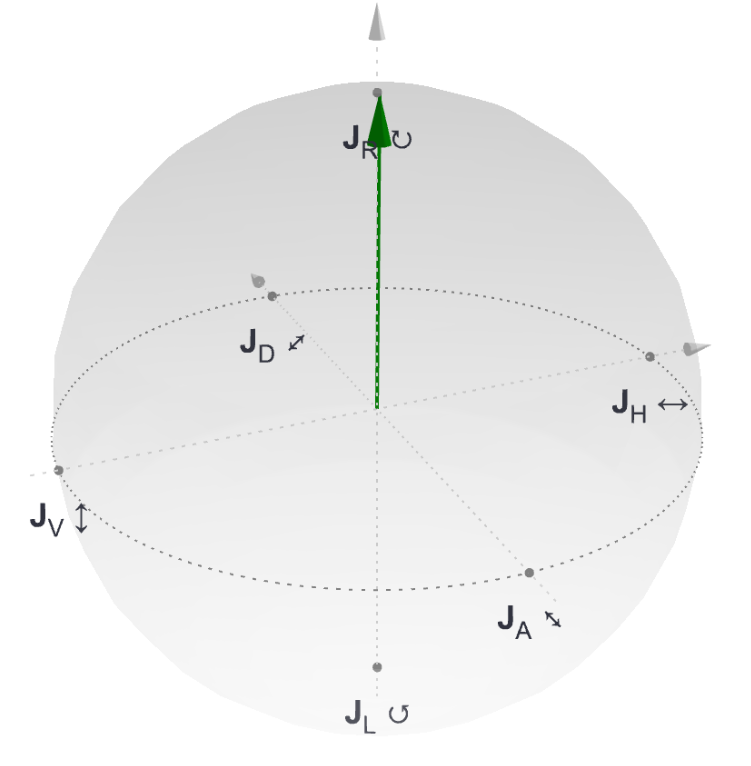
\includegraphics[width=\textwidth]{images/poincare.png}
\end{columns}
\slidesource{Polarisations-Applet GitHub \citep{2026polarization}}
\note{Bei Standard-Pauli-Matrizen-Reihenfolge für denselben Zweikomponentenzustand lautet der Bloch-Vektor (S2,S3,S1). Die Bezeichnungen für zirkulare Polarisation hängen von Ausbreitungs- und Phasenkonventionen ab. Behalten Sie während der gesamten Präsentation die Konvention des Applets bei.}
\end{frame}

%\begin{frame}{Was der geometrische Zusammenhang zeigt – und was nicht}
%\begin{itemize}
%\item Nach Wahl einer Basis- und Achsenkonvention teilen reine Qubit-Zustände und normierte Jones-Zustände dieselbe Kugelgeometrie.
%\item Eine globale Phase verändert den dargestellten Zustand nicht.
%\item Eine verlustfreie Verzögerungsplatte ändert den Zustand ohne Intensitätsverlust.
%\item Ein Polarisator ändert den transmittierten Zustand und verringert in der Regel die Intensität. Die Kugel allein kodiert diese Intensität nicht.
%\end{itemize}
%\keyidea{Die didaktische Herausforderung besteht darin, einen mathematischen Zustandsraum zu interpretieren, ohne ihn zu einem wörtlichen physischen Objekt zu machen.}
%\source{Implementierung des Jones-Kalküls und didaktische Begründung.}
%\note{Bei einer transmittierten Intensität von null ist ein normierter Ausgangs-Polarisationszustand nicht definiert. Vermeiden Sie es, einen Punkt auf der Kugel so zu verwenden, als hätte ein ausgelöschtes Feld eine messbare Polarisation. Diese Präsentation erhebt nicht den Anspruch, dass klassische Polarisation alle Quantenphänomene reproduziert.}
%\end{frame}

\subsection{Bedingungen und Aufgaben}
\begin{frame}{Das Applet}
\begin{columns}[T,onlytextwidth]
\column{0.48\textwidth}
\centering
\textbf{Kontrollgruppe:} \\ Jones-Notation und Wellengraph.
\column{0.48\textwidth}
\centering
\textbf{Experimentalgruppe:} \\ Zusätzlich mit Poincar\'e-Kugel.
\end{columns}
\centering
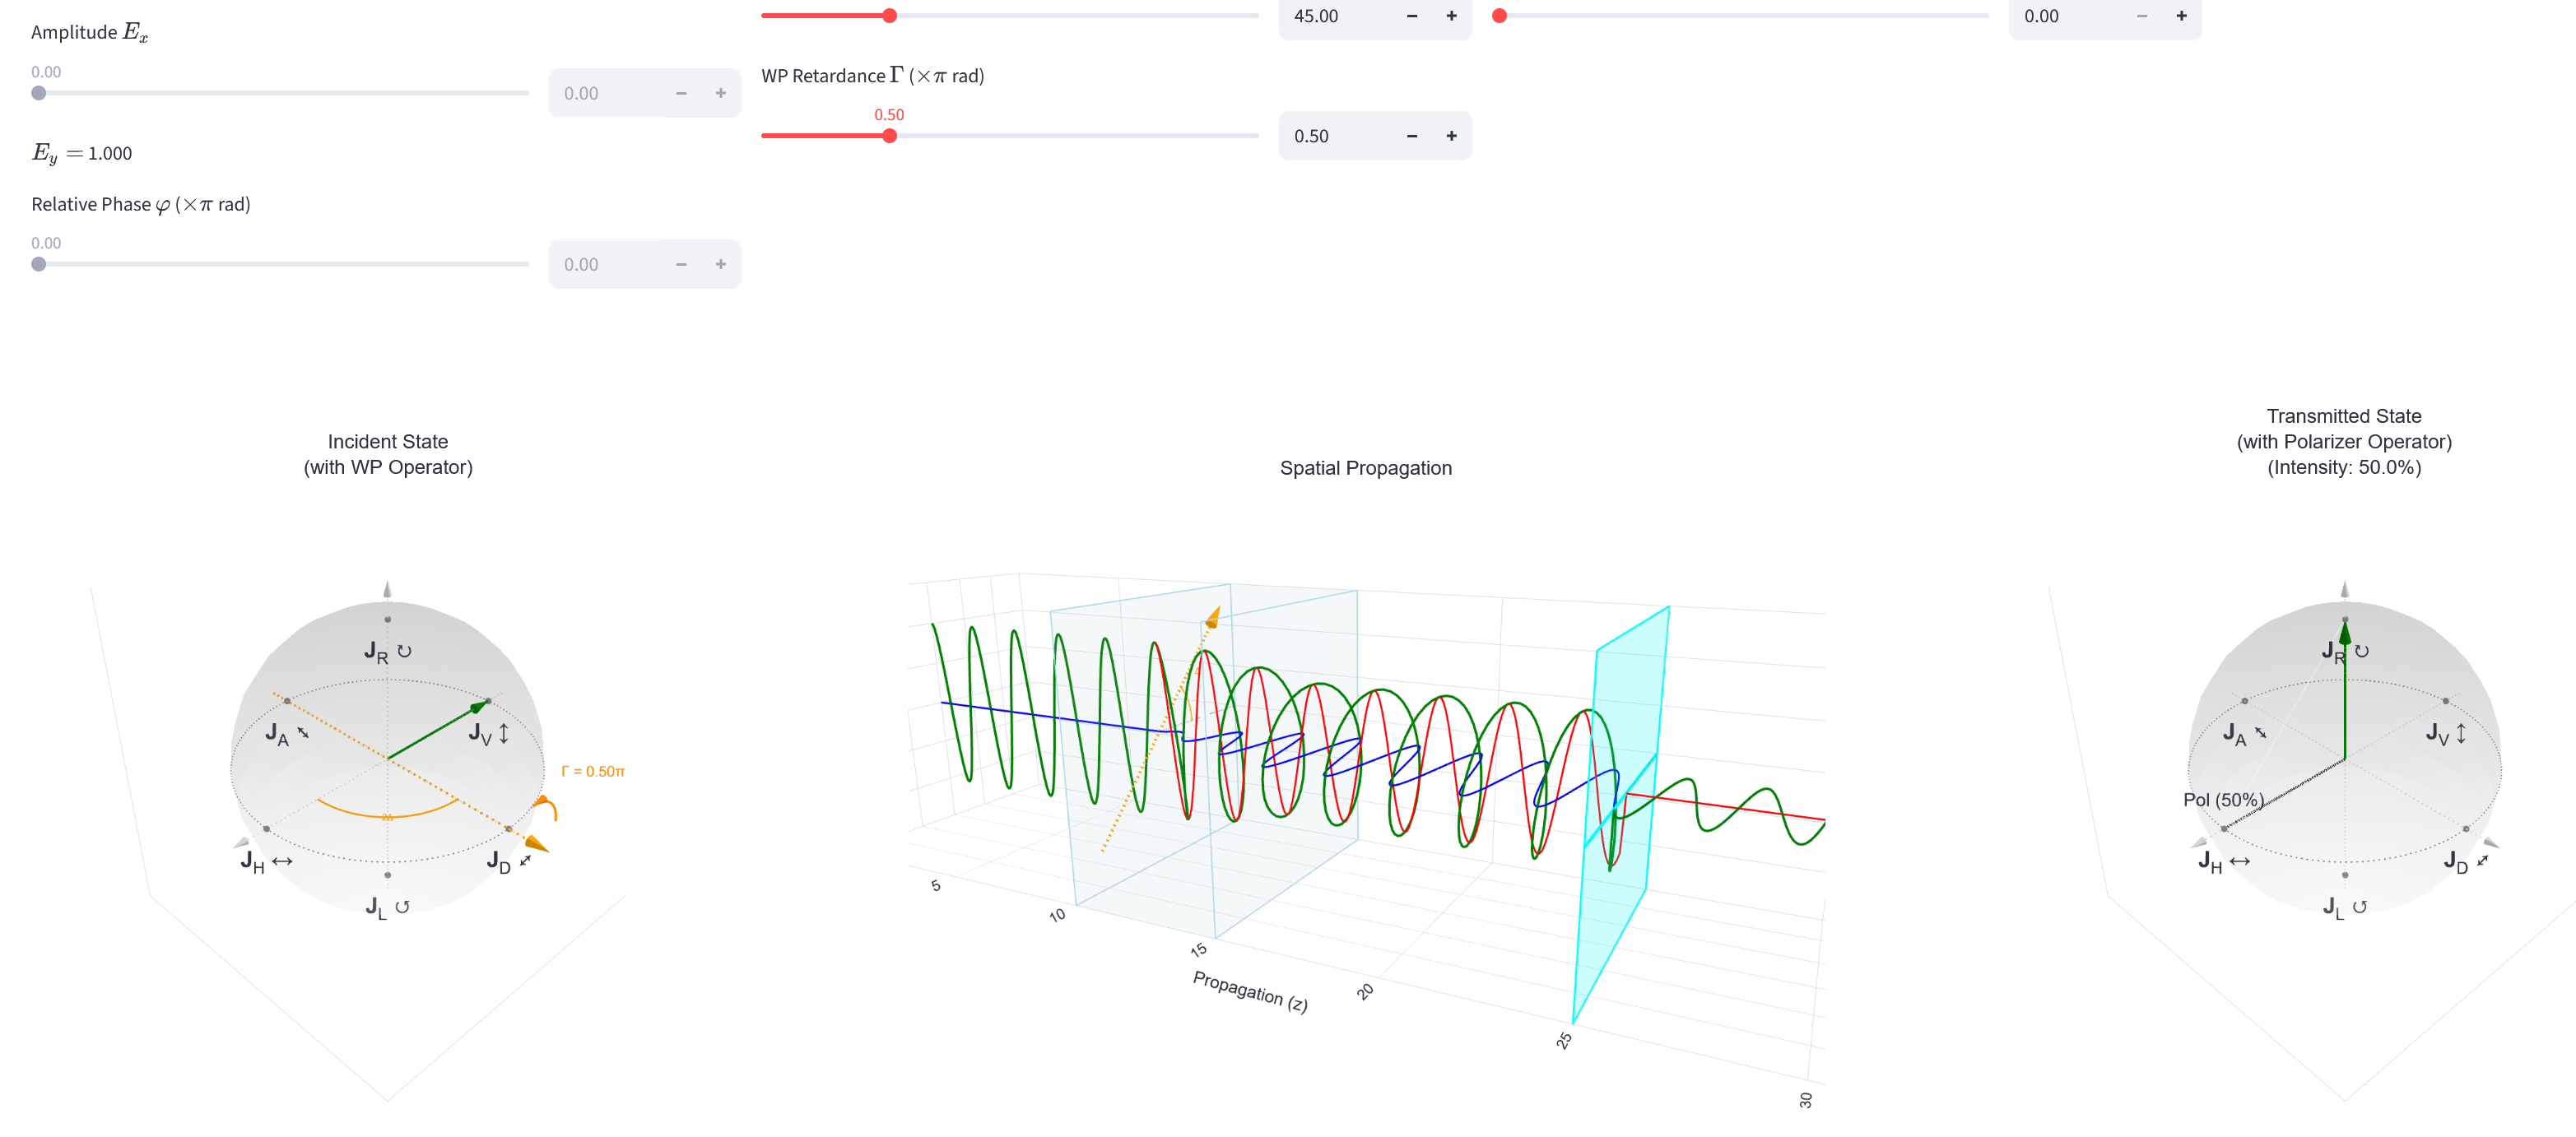
\includegraphics[width=0.82\textwidth]{images/applet.png}

{\small + Einführende Erklärungen, angeleitete Parameteränderungen, Hinweise und Lösungen.}
% \source{Condition mapping and timing: \texttt{app.py} and \texttt{challenges.py}.}
\slidesource{Polarisations-Applet GitHub \citep{2026polarization}}
\note{Verwenden Sie Screenshots desselben optischen Zustands und Schritts. Die aktuellen Versionen unterscheiden sich auch im instruktionalen Wortlaut und in einem anfänglichen Winkel der Verzögerungsplatte. Siehe den Implementierungsanhang, bevor der Kontrast als rein visuelle Manipulation beschrieben wird.}
\end{frame}

\begin{frame}{Die Lernsequenz}
\begin{tabularx}{\textwidth}{@{}P{0.12\textwidth}P{0.31\textwidth}Y@{}}
\toprule
\textbf{Schritte} & \textbf{Thema} & \textbf{Lernaktivität} \\
\midrule
1--3 & Polarisationszustände & Amplituden und relative Phase ändern, um lineare und zirkulare Zustände zu erzeugen. \\
4--6 & Verzögerungsplatten & Verzögerung und schnelle Achse variieren, um einen Zustand zu transformieren. \\
7 & Lineare Polarisatoren & Orientierung der Transmissionsachse mit der Ausgangsintensität verknüpfen. \\
8--9 & Kombinierte Operatoren & Verzögerungsplatten und Polarisatoren koordinieren, um einen Zielzustand zu erreichen. \\
\bottomrule
\end{tabularx}\par
\vspace{2.5mm}
Neun Aufgaben (Challenges) gehen dem Abschlussbildschirm und dem Link zurück zur Umfrage voraus.
% \source{Challenge definitions. A revealed solution can also satisfy the target.}
\end{frame}
